\documentclass{standalone}

\usepackage{tikz}

\begin{document}
  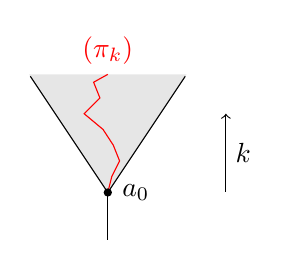
\begin{tikzpicture}
    \draw[opacity=0.2,fill=gray,draw=none] (0,0) -- (1,1.5) -- (-1,1.5) to (0,0);
    \node[inner sep=0pt] (b) at (-1,1.5) {};
    \node[inner sep=0pt] (c) at (1,1.5) {};
    \draw (b) -- (0,0);
    \draw (c) -- (0,0);
    \draw (0,0) -- (0,-0.6);
    % Random path inside the triangle
    \draw[red] (0,0) -- (0.05,0.2) -- (0.15,0.4) -- (0.07,0.6) -- (-0.06,0.8) -- (-0.3,1) -- (-0.1,1.2) -- (-0.18,1.4) -- (0,1.5);
    \node[red] at (0,1.8) {$(\pi_k)$};
    \node[circle,fill=black,inner sep=0pt,minimum size=3pt, label=right:{$a_0$}] (a) at (0,0) {};
    \draw[<-] (1.5,1) -- (1.5,0) node[midway, right] {$k$};
  \end{tikzpicture}
\end{document}